\documentclass{standalone}

\usepackage{tikz,pgfplots,textcomp}
\usetikzlibrary{calc,arrows.meta}

\begin{document}
  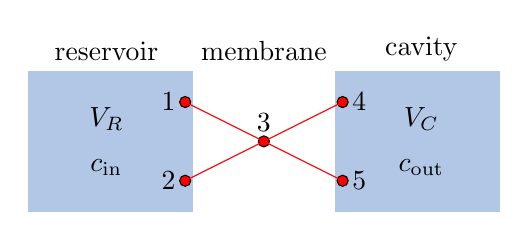
\begin{tikzpicture}[>=Latex]

    \newlength\plotwidth\setlength{\plotwidth}{8cm}
\newlength\plotheight\setlength{\plotheight}{5cm}
\newlength{\margX}\setlength{\margX}{1.8cm}
\newlength{\margY}\setlength{\margY}{1.3cm}
\def\legendfontsize{8}
\def\labelfontsize{10}
\def\legfont{\fontsize{\legendfontsize}{\legendfontsize}\selectfont}
\def\labfont{\fontsize{\labelfontsize}{\labelfontsize}\bf\selectfont}
\def\smalldpi{100}
\def\lwidth{1}
\newlength\wdth

\definecolor{clr1}{rgb}{0.00,0.30,0.80} 
\definecolor{clr2}{rgb}{0.90,0.30,0.00} 
\definecolor{clr3}{rgb}{0.00,0.70,0.00} 
\definecolor{clr4}{rgb}{0.65,0.00,0.65} 
\definecolor{clr5}{rgb}{0.00,0.00,0.00} 
\definecolor{clr6}{rgb}{0.60,0.60,0.60} 
\definecolor{lblue}{rgb}{0.7,0.78,0.9}
\definecolor{lgray}{rgb}{0.75,0.75,0.75}
\definecolor{dds}{rgb}{0.19,0.47,0.56} 

\coordinate (p1) at (0,0);
\coordinate (p2) at ($(p1)+(\plotwidth+\margX,0)$);
\coordinate (p3) at ($(p1)+(0,-\plotheight-\margY)$);
\coordinate (p4) at ($(p3)+(\plotwidth+\margX,0)$);
\coordinate (p5) at ($(p3)+(0,-\plotheight-\margY)$);
\coordinate (p6) at ($(p5)+(\plotwidth+\margX,0)$);
\coordinate (p7) at ($(p5)+(0,-\plotheight-\margY)$);
\coordinate (p8) at ($(p7)+(\plotwidth+\margX,0)$);
\coordinate (p9) at ($(p7)+(0,-\plotheight-\margY)$);
\coordinate (p10) at ($(p9)+(\plotwidth+\margX,0)$);
\coordinate (p11) at ($(p9)+(0,-\plotheight-\margY)$);
\coordinate (p12) at ($(p11)+(\plotwidth+\margX,0)$);
\coordinate (p13) at ($(p11)+(0,-\plotheight-\margY)$);

\pgfplotsset{
  compat=1.15,
  legend pos=south east,
  legend cell align = left,
  width=\plotwidth, height=\plotheight, scale only axis,
  y label style={font={\labfont}},
  x label style={font={\labfont}},
  x tick label style={font=\fontsize{\legendfontsize}{\legendfontsize}\selectfont},
  y tick label style={font=\fontsize{\legendfontsize}{\legendfontsize}\selectfont},
  legend style={font=\fontsize{\legendfontsize}{\legendfontsize}\selectfont},
  /pgf/number format/.cd,
  1000 sep={}
  }
    \setlength\wdth{5cm}

    \coordinate (n1) at (0,1);
    \coordinate (n2) at (0,0);
    \coordinate (n3) at (1,0.5);
    \coordinate (n4) at (2,1);
    \coordinate (n5) at (2,0);

    \fill[color=lblue] (-2,-0.4) rectangle (0.1,1.4);
    \fill[color=lblue] (4,-0.4) rectangle (1.9,1.4);

    \foreach \x in {1,2,...,5}{
      \draw[fill=red] (n\x) circle (2pt);
    }

    \foreach \x in {1,2}{
      \node[left] at (n\x){$\x$};
    }
    \node[above] at (n3){$3$};
    \foreach \x in {4,5}{
      \node[right] at (n\x){$\x$};
    }

    \node[above] at (3,1.4){cavity};
    \node[above] at (1,1.4){membrane};
    \node[above] at (-1,1.4){reservoir};
    \node[align=center] at (-1,0.5){$V_R$\\[1ex]$c_{\rm in}$};
    \node[align=center] at (3,0.5){$V_C$\\[1ex]$c_{\rm out}$};

    \draw[red] (n1) -- (n3) -- (n4);
    \draw[red] (n2) -- (n3) -- (n5);


  \end{tikzpicture}
\end{document}